\documentclass[11pt]{scrartcl}
\usepackage[sexy]{../../../evan}
\usepackage{graphicx}

\definecolor{dg}{RGB}{2,101,15}
\newtheoremstyle{dotlessP}{}{}{}{}{\color{dg}\bfseries}{}{ }{}
\theoremstyle{dotlessP}
\newtheorem{property}[theorem]{Property}

\newtheoremstyle{dotlessN}{}{}{}{}{\color{teal}\bfseries}{}{ }{}
\theoremstyle{dotlessN}
\newtheorem{notation}[theorem]{Notation}
% Shortcuts
\DeclarePairedDelimiter\ceil{\lceil}{\rceil} % ceil function

\DeclarePairedDelimiter\paren{(}{)} % parenthesis

\newcommand{\df}{\displaystyle\frac} % displaystyle fraction
\newcommand{\qeq}{\overset{?}{=}} % questionable equality

\newcommand{\Mod}[1]{\;\mathrm{mod}\; #1} % modulo operator

\newcommand{\comp}{\circ} % composition

% Text Modifiers
\newcommand{\tbf}{\textbf}
\newcommand{\tit}{\textit}

% Sets
\DeclarePairedDelimiter\set{\{}{\}}
\newcommand{\unite}{\cup}
\newcommand{\inter}{\cap}

\newcommand{\reals}{\mathbb{R}} % real numbers: textbook is Z^+ and 0
\newcommand{\ints}{\mathbb{Z}}
\newcommand{\nats}{\mathbb{N}}
\newcommand{\complex}{\mathbb{C}}
\newcommand{\tots}{\mathbb{Q}}

\newcommand{\degree}{^\circ}

% Counting
\newcommand\perm[2][^n]{\prescript{#1\mkern-2.5mu}{}P_{#2}}
\newcommand\comb[2][^n]{\prescript{#1\mkern-0.5mu}{}C_{#2}}

% Relations
\newcommand{\rel}{\mathcal{R}} % relation

\setlength\parindent{0pt}

% Directed Graphs
\usetikzlibrary{arrows}
\tikzset{vertex/.style = {shape=circle,draw,minimum size=2em}}
\tikzset{svertex/.style = {shape=circle,draw,minimum size=.05em,font=\tiny}}
\tikzset{edge/.style = {->,> = latex'}}
\tikzset{dedge/.style = {-> = latex'}}
\tikzset{dot/.style={inner sep=1.5pt,circle,draw,fill}}


% Contradiction
\newcommand{\contradiction}{{\hbox{%
    \setbox0=\hbox{$\mkern-3mu\times\mkern-3mu$}%
    \setbox1=\hbox to0pt{\hss$\times$\hss}%
    \copy0\raisebox{0.5\wd0}{\copy1}\raisebox{-0.5\wd0}{\box1}\box0
}}}

\newcommand{\xxhash}[2]{\rotatebox[origin=c]{#2}{$#1\parallel$}}

\title{CS 120: Intro to Algorithms and their Limitations}
\subtitle{PSet 3}
\author{Denny Cao}
\date{\today}
%++++++++++++++++++++++++++++++++++++++++
% title stuff
\usepackage{titling}
\renewcommand\maketitlehooka{\null\mbox{}\vfill}
\renewcommand\maketitlehookd{\vfill\null}
\makeatletter
\renewcommand{\maketitle}{\bgroup\setlength{\parindent}{0pt}
	\begin{flushleft}
		\large\textbf{\@title} \\ \vskip 0.2cm
		\begingroup
		\fontsize{14pt}{12pt}\selectfont
		\title
		\\
		Problem Set 3
		\endgroup \vskip 0.3cm
		Due: October 4, 2023 11:59pm \hfill\rlap{}\textbf{Denny Cao} \\ \vskip 0.1cm
		\hrulefill
	\end{flushleft}\egroup
}
\makeatother

\renewcommand{\theques}{\thesection.\alph{ques}} % Change subtheo counter for alpha output
\declaretheorem[style=basehead,name=Answer,sibling=theorem]{ans}
\renewcommand{\theans}{\thesection.\alph{ans}}
\begin{document}
\maketitle
\pagestyle{plain}
\textbf{Collaborators:}

\textbf{No. of late days used on previous psets:} 0

\textbf{No. of late days used after including this pset:} 1
\stepcounter{section}
\section{Empirically Evaluating Simulation Runtimes and Explaining Them Theoretically}
\begin{enumerate}[(a)]
	\item Let $P_1(x)$ and $P_2(x)$ denote the outputs of the first and second program respectively given an input $x$. Then, $\text{Time}_{P_1}(N) = 10 + 4N$ and $\text{Time}_{P_2}(N) = 14 + 7N$.
		\\

		We obtain this by observing that the first program executes 7 commands from lines 0 to 6 before entering a loop that executes 4 commands from lines 7 to 10 $N$ times. The last time the loop runs, it will go back to line 7 which will exit the loop to line 11, executing another command. The program then executes 2 more commands from lines 11 to 12, giving us a total of $\text{Time}_{P_1}(N) = 7 + 4N + 1 + 2 =  10 + 4N $.
		\\

		For the second program, there are 8 commands before entering a loop that executes 7 commands from lines 8 to 14 $N$ times. The last time the loop runs, it will go back to line 8 which will exit the loop to line 15, executing another command. The program then executes 5 more commands from lines 15 to 19, giving us a total of $\text{Time}_{P_2}(N) = 8 + 7N + 1 + 5 = 14 + 7N$.
		\\

		As $10 + 4N < 14 + 7N$, Program 1 runs faster for all $N \in \nats$.
	\item Program 2 is faster. However, for smaller inputs than 12, Program 1 is faster. At $N \geq 12$, Program 2 is faster.
		\begin{center}
			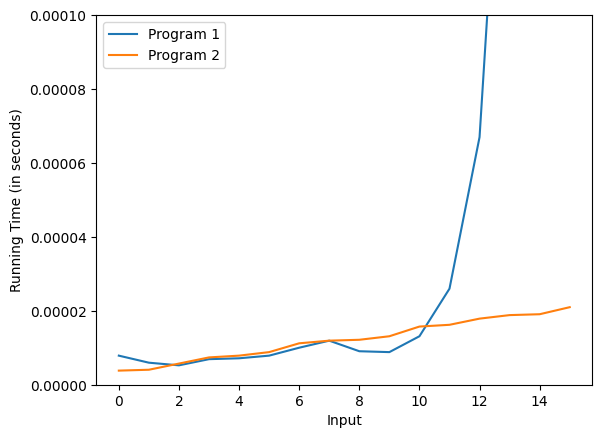
\includegraphics[width=0.75\textwidth]{running_times.png}
		\end{center}
	\item The discrepancies we see between Parts 2a and 2b are due to the assumption in the RAM model that every operation takes $O(1)$ time. However, in reality, as the numbers in the programs grow large rapidly, the time it takes for each operation will depend on the size of the input. This is only an issue in Program 1, as the value of \texttt{result} is not bounded and will grow exponentially large and will quickly exceed the limit that can be stored in a word, requiring multiple words to store the value of \texttt{result}. This creates the exponential curve we see in (2b) rather than the linear curve we expect to see in (2a). In contrast, Program 2 bounds the value of \texttt{result} by taking $\texttt{result}\text{ mod }{2^{32}}$ in every iteration of the loop, allowing $\texttt{result}$ to be stored in one word, and thus the operations on $\texttt{result}$ for Program 2 can be $O(1)$ which is why Program 2 is linear both in (2a) and (2b).
	\item We can bound the runtime by observing the true runtime of the multiplication operator. In Python, when multiplying large numbers, \href{https://hg.python.org/cpython/file/b514339e41ef/Objects/longobject.c#l2694}{Karatsuba multiplication} is used, which runs in \href{https://brilliant.org/wiki/karatsuba-algorithm/#:~:text=Using%20the%20master%20theorem%20on,%E2%89%88%20%CE%98%20(%20n%201.585%20)%20.}{$O(N^{\log_{2}3})$} where $N$ is the maximum number of bits of the factors.
		\\

		For Program 2, the maximum number that is multiplied is  $2^{32}$. Thus, multiplication would run in  $O\paren*{\paren*{2^{32}}^{\log_2{3}}} = O\paren*{\paren*{2^{\log_2{3}}}^{32}} = O(3^{32}) = O(1)$ time, and thus multiplication takes constant time, resulting in the linear curve we see in (b), as multiplication is computed $n$ times, resulting in $O(n)$.
		\\

		For Program 1, the largest multiplication executed is $17^{2^n} \times 17$. Thus, we can bound the runtime of Program 1 by overestimating the runtime for multiplication as the runtime it takes to execute $17^{2^n} \times 17$. The maximum number of bits of the factors is $\log_2 {17^{2^n}} = 2^n \paren*{\log_2 17}$. Thus, with Karatsuba multiplication, the runtime will be $O\paren*{\paren*{2^n{\log_2 17}}^{\log_2 3}} = O\paren*{\paren*{2^n}^{\log_2 3}\paren*{\log_2 17}^{\log_2 3}} = O\paren*{3^n \paren*{\log_2 17}^{\log_2 3}}$. As $\paren*{\log_2 17}^{\log_2 3}$ is a constant,  $O\paren*{3^n \paren*{\log_2 17}^{\log_2 3}} = O(3^n)$. As multiplication is computed $n$ times, the runtime of Program 2 can be bounded by  $O(n 3^n)$, creating the exponential curve we see in (b).
\end{enumerate}
\section{Simulating Word-RAM by RAM}
		\begin{proof} We will take a simulation strategy by using an implementation-level description.
			\\

			\textbf{Computability (Operations)}:
			\begin{enumerate}[(i)]
				\item \textbf{Initialization}:
			In $P'$, compute variables \texttt{word\_len} and \texttt{mem\_size}. 

			As \texttt{mem\_size} is the length of the input, we set $\texttt{mem\_size} = \texttt{input\_len}$.  Then, \texttt{word\_len} can be computed as follows:
			\[
				\texttt{word\_len} = \floor{\log \max \set*{\texttt{mem\_size}, x[0], \dots , x[n-1]}} + 1
			\] 
			We can break computing \texttt{word\_len} into two parts. For the first part, we find the largest element of the $n$ inputs. We can implement this in a RAM Program by iterating over the $n$ inputs and creating a variable \texttt{max} that stores the current maximum element, making comparisons between the current input element and \texttt{max}, setting \texttt{max} to the current input element if the element is larger than \texttt{max}. At the end of the loop, \texttt{max} will be the largest element of the $n$ input elements and can then be compared to \texttt{mem\_size} to see which is larger. Let this value be $k$.


			For the second part, the length of $k$ can be found by computing $\floor{\log_2 {k}}$, which we can implement in a RAM Program by continually setting $k = \floor{\frac{k}{2}}$ until  $k = 0$ and counting how many divisions are needed. We then add 1 to this value to obtain \texttt{word\_len}.


			For convenience, we compute $\texttt{max\_num} = 2^{\texttt{word\_len}}$. We implement this in a RAM Program by setting \texttt{max\_num} to 1 and then setting a variable \texttt{temp} to \texttt{word\_len}. Then, multiply \texttt{max\_num} by 2 and then decrement \texttt{temp} by 1 and then repeat until \texttt{temp==0}.

		\item \textbf{Memory}: In $P'$, when reading and writing to memory locations larger than \texttt{mem\_size}, nothing occurs. We can implement this in a RAM Program by adding an additional check to the read and write operations to check if, for the memory location $M[i]$, if  $i \leq \texttt{mem\_size}$, and if it is, then continue with the operation. By doing so, if the memory location is greater than \texttt{mem\_size}, nothing will occur.
		\item \textbf{Operations}: All operations are the same as $P$, but the addition and multiplication operations are redefined to return $2^{w_0} - 1$ if the result is $\geq 2^{w_0}$. We can implement this in a RAM Program by checking if the result of the addition and multiplication operation is greater than \texttt{max\_num}. Let $\texttt{var}_i = \texttt{var}_j + \texttt{var}_k$ or $\texttt{var}_i = \texttt{var}_j \times \texttt{var}_k$. Then, after computing the operation, check if $\texttt{var}_i \geq \texttt{max\_num}$, and if it is, set $\texttt{var}_i = \texttt{max\_num} - 1$.
		\item \textbf{MALLOC}: In $P'$, \texttt{MALLOC} is an operation that increases memory size beyond \texttt{mem\_size}. We can implement this in a RAM Program by incrementing \texttt{mem\_size} by 1, setting $M[\texttt{mem\_size} - 1] = 0$, and if $\texttt{mem\_size} = 2^{\texttt{word\_len}}$, it also increments \texttt{word\_len} by 1. We also double \texttt{max\_num} by 2 in order to maintain the fact that $\texttt{max\_num} = 2^{\texttt{word\_len}}$.
\end{enumerate}
			\textbf{Runtime (Operations)}: 
			\begin{enumerate}[(i)]
				\item \textbf{Initialization}:
					When computing \texttt{word\_len}, the first part we discussed in the operation is done by iterating through the $n$ input elements and drawing a comparison between the element and the \texttt{max} variable, taking $O(n)$ time. For the second part, if  $k$ can be represented in $w_0$ bits, then $k \leq 2^{w_0} - 1$. Thus,  $\floor{\log_2 k} \leq w_0 - 1$, meaning that we will have to do at most $w_0$ divisions before exiting the loop. As all other operations take $O(1)$ time in our implementation of the second part, it will take $O(w_0)$ time to compute the second part. Thus, in total, to compute \texttt{word\_len}, it takes $O(n + w_0)$ time. When setting $\texttt{mem\_size} = \texttt{input\_len}$, reading from memory takes  $O(1)$ time. Computing \texttt{max\_num} is done through a loop that computes basic operations \texttt{word\_len} times, and thus takes $O(w_0)$ time. Thus, the initialization of $P'$ can be bounded by  $O(n + w_0)$ time.
				\item \textbf{Memory}: For read and write operations, an additional check is needed to check if the memory location is less than or equal to \texttt{mem\_size}, which will take  $O(1)$ time.
				\item \textbf{Operations}: For addition and multiplication operations, an additional check is needed at the end of the operation to check if the result is greater than or equal to \texttt{max\_num} which takes $O(1)$ time and if it is, then set it to $\texttt{max\_num} - 1$, which takes $O(1)$ time.
				\item \textbf{MALLOC}: Incrementing, setting, and multiplying are all basic operations and thus can be done in $O(1)$ time.
\end{enumerate}
\item \textbf{Computability (Program)}: For every Word-RAM program $P$, there is an ordinary RAM program $P'$ that performs the same operations, except it replaces every operation specified in \textbf{Computability (Operations)} with the corresponding substitute. We have shown that our simulated Word-RAM program is equivalent to the original Word-RAM program, as we have shown substitutes for the differences and kept all other operations the same. Thus, for every Word-RAM program $P$, there exists a modified RAM program $P'$ that will have the same output as $P$ on every input $x$. Thus, if $P'$ halts on $x$ $\iff$  $P$ halts on $x$, and if they halt, then $P(x) = P'(x)$, and the first part of the theorem is proven.
	\\

	\textbf{Runtime (Program)}: Every change we made to an operation took a constant number of steps, and thus is  $O(1)$. The initialization step takes $O(n + w_0)$ time, and thus our overall time is:
	\begin{align*}
		T_{P'}(x) &= O(1)(T_P(x)) + O(n + w_0) \\
				  &= O(T_P(x) + n + w_0)
	\end{align*}
		and the second part of the theorem is proven.
		\end{proof}
\end{document}
